\documentclass[a4paper,11pt]{article}
\usepackage[utf8]{inputenc}
\usepackage{amsmath}
\usepackage{amssymb}
\usepackage{geometry}
\usepackage{graphicx}
\usepackage{float}
\usepackage{fancyhdr}

\geometry{a4paper, margin=1in}

\title{Exercice 3: Beaux Rivages}
\author{SANNA Thomas, L3STI}
\date{\today}

% Configuration des en-têtes et pieds de page
\pagestyle{fancy}
\fancyhf{}
\fancyhead[L]{Conception de BDD}
\fancyhead[C]{Exercice 3: Beaux Rivages}
\fancyhead[R]{\today}
\fancyfoot[C]{Page \thepage}
\fancyfoot[L]{SANNA Thomas, L3STI}
\fancyfoot[R]{Università di Corsica Pasquale Paoli}

\begin{document}

\maketitle

\section{Recensement des attributs}
À partir de l'image donné pour l'exercice, nous avons identifié les attributs suivants pour chaque entité:

\begin{figure}[H] 
    \centering
    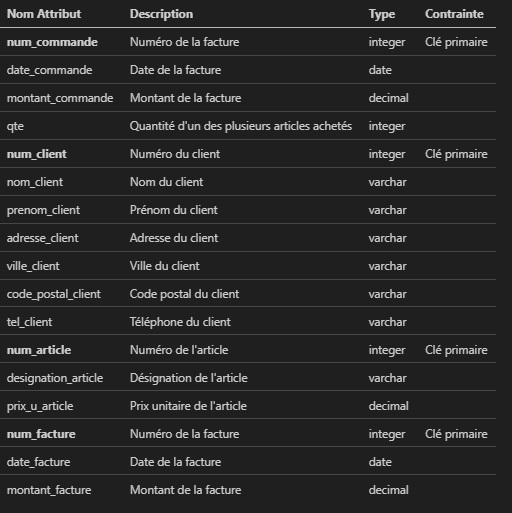
\includegraphics[width=0.8\textwidth]{image.png}
    \caption{Rescensement des attributs. Table effectuée à l'aide de MarkDown}
    \label{fig:image}
\end{figure}

\subsection*{Contraintes}
\begin{itemize}
    \item Une commande ne peut être passée que par un seul client.
    \item Un client peut passer plusieurs commandes.
    \item Une commande peut contenir plusieurs articles.
    \item Un article peut apparaître dans plusieurs commandes.
    \item Une facture ne peut être associée qu'à une seule commande.
    \item Une commande ne peut être associée qu'à une seule facture.
\end{itemize}

\section{Dépendances fonctionnelles}
Les dépendances fonctionnelles identifiées pour chaque entité sont:

$\texttt{num\_commande} \to \{\text{date\_commande, montant\_commande, num\_client, num\_facture}\}$

$\texttt{num\_client} \to \{\text{nom\_client, prenom\_client, adresse\_client, ville\_client, code\_postal\_client, tel\_client}\}$

$\texttt{num\_article} \to \{\text{designation\_article, prix\_u\_article}\}$

$\texttt{num\_facture} \to \{\text{date\_facture, montant\_facture\_ht}\}$

$\texttt{num\_commande, num\_article} \to \{\text{qte}\}$

\section{Diagramme des attributs}
\begin{figure}[H] 
    \centering
    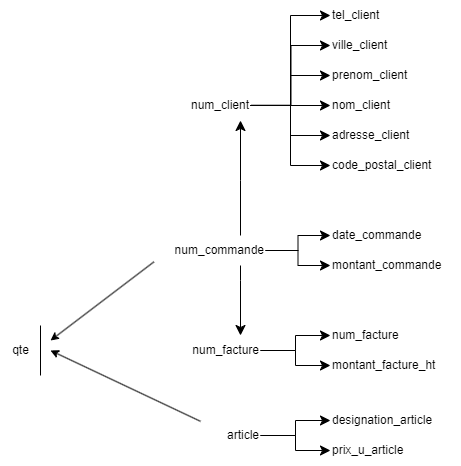
\includegraphics[width=0.7\textwidth]{attributs.png}
    \caption{Diagramme des attributs}
    \label{fig:attributs}
\end{figure}

\break\section{Couverture minimale}

\begin{enumerate}
    \item \textbf{Élimination des attributs redondants}: Nous ne trouvons pas d'attributs redondants dans les dépendances fonctionnelles actuelles.
    \item \textbf{Réduction du côté gauche des dépendances}: Chaque attribut du côté gauche est indispensable pour déterminer les attributs du côté droit.
    \item \textbf{Décomposition du côté droit}: Les dépendances fonctionnelles ne nécessitent pas de décomposition, car chaque dépendance a un ensemble minimal d'attributs.
\end{enumerate}

Ainsi, la couverture minimale des dépendances fonctionnelles reste inchangée.

\section{Conception du Modèle Conceptuel de Données (MCD)}

\begin{enumerate}
    \item \textbf{Définition de l’ensemble des identifiants}: 
    \begin{itemize}
        \item Commande: \texttt{num\_commande}
        \item Client: \texttt{num\_client}
        \item Article: \texttt{num\_article}
        \item Facture: \texttt{num\_facture}
    \end{itemize}
    \item \textbf{Recherche des entités}:
    \begin{itemize}
        \item Commande
        \item Client
        \item Article
        \item Facture
    \end{itemize}
    \item \textbf{Recherche des relations}:
    \begin{itemize}
        \item$Commande \rightarrow Client: (1,1)$
        \item $Commande \rightarrow Article: (1,N)$
        \item $Commande \rightarrow Facture: (1,1)$
        \item $Facture \rightarrow Commande: (1,N)$
        \item $Client \rightarrow Commande: (0,N)$
        \item $Article \rightarrow Commande: (0,N)$
    \end{itemize}
\end{enumerate}

\section{Schéma Relationnel}

\begin{itemize}
    \item \textbf{Commande} (\underline{num\_commande}, date\_commande, montant\_commande, num\_client, num\_facture)
    \item \textbf{Client} (\underline{num\_client}, nom\_client, prenom\_client, adresse\_client, ville\_client, code\_postal\_client, tel\_client)
    \item \textbf{Article} (\underline{num\_article}, designation\_article, prix\_u\_article)
    \item \textbf{Facture} (\underline{num\_facture}, date\_facture, montant\_facture\_ht)
    \item \textbf{Commande\_Article} (\underline{num\_commande}, \underline{num\_article}, qte)
\end{itemize}

\subsection*{Contraintes d'intégrité}
\begin{itemize}
    \item \textbf{Commande}:
    \begin{itemize}
        \item \texttt{num\_client} est une clé étrangère référencée par \texttt{Client(num\_client)}
        \item \texttt{num\_facture} est une clé étrangère référencée par \texttt{Facture(num\_facture)}
    \end{itemize}
    \item \textbf{Commande\_Article}:
    \begin{itemize}
        \item \texttt{num\_commande} est une clé étrangère référencée par \texttt{Commande(num\_commande)}
        \item \texttt{num\_article} est une clé étrangère référencée par \texttt{Article(num\_article)}
    \end{itemize}
\end{itemize}

\section{Modèle Conceptuel de Données (MCD)}
\begin{figure}[H] 
    \centering
    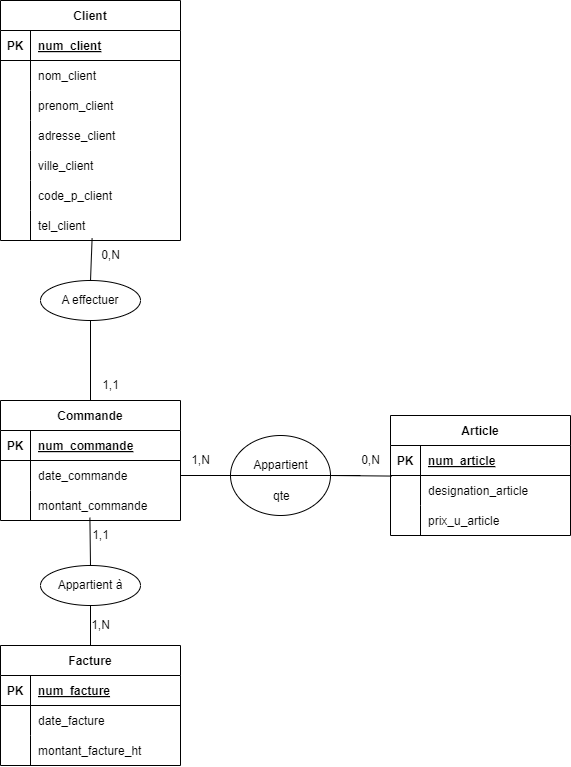
\includegraphics[width=0.8\textwidth]{exo4-mcd.png}
    \caption{Modèle Conceptuel de Données (MCD)}
    \label{fig:mcd}
\end{figure}

\end{document}